\documentclass[11pt]{article}
\usepackage{graphicx} % This lets you include figures
\usepackage{hyperref} % This lets you make links to web locations
\usepackage[margin=0.5in]{geometry}
\usepackage[rightcaption]{sidecap}
\usepackage{subcaption}
\usepackage{wrapfig}
\usepackage{float}
\usepackage{imakeidx}
\usepackage{indentfirst}
\makeindex
%---------------------------Do Not Edit Anything Above This Line!!------------------------

% edit the line below, if needed, to change the directory name for your image files.
\graphicspath{ {./images/} }



\begin{document}

%---------------------------Edit Content in the Box to Create the Title Page--------------
\begin{titlepage}
   \begin{center}
       \vspace*{1cm}
	   \Huge
       \textbf{Star Wars}

       \vspace{0.5cm}
       \Large
       Sprint 3\\
       November 3rd, 2023 \\
   \end{center}

       \vspace{1.5cm}

\begin{table}[h!]
\centering
\begin{tabular}{|l|l|}
\hline
\textbf{Name} & \textbf{Email Address} \\ \hline
Matthew Irizarry         & matthew.irizarry745@topper.wku.edu         \\ \hline
Zach Vance         & zachary.vance141@topper.wku.edu         \\ \hline
Keimon Bush         & keimon.bush105@topper.wku.edu        \\ \hline
Jeremiah Harris         & jeremiah.harris978@topper.wku.edu         \\ \hline
\end{tabular}
\end{table}

%Latex Table Generator    
%https://www.tablesgenerator.com/     
        
\vspace{4in}

\centering        
CS 360 \\
Fall 2023\\
Project Technical Documentation

\end{titlepage}
%---------------------------Edit Content in the Box to Create the Title Page--------------


% No text here.


%---------------------------Do Not Edit Anything In This Box!!------------------------
%Table of contents and list of figures will be autogenerated by this section.
\newpage
\setcounter{page}{1}%
\cleardoublepage
\pagenumbering{gobble}
\tableofcontents
\cleardoublepage
\pagenumbering{arabic}
\clearpage
\newpage
\setcounter{page}{1}%
\cleardoublepage
\pagenumbering{gobble}
\listoffigures
\cleardoublepage
\pagenumbering{arabic}
\newpage
%---------------------------Do Not Edit Anything In This Box!!------------------------




%---------------------------Project Introduction Section------------------------------

% No text here.

\section{Introduction} %\section{} is used to create major section headers

% No text here.

%---------------------------Project Overview------------------------------------------
\subsection{Project Overview} %\subsection{} is used to create minor sections 
% 300 words
% Description of the project, what the project provides, its purpose, problems solved, and target audience.

This project will attempt to produce a recreation of the 1991 Star Wars game that was produced for the SEGA Master System. While we will not be recreating every level and aspect of the game, the aim is to create a fun, quality homage to the original. This means that at the end of delivery, the game should have minimal bugs, be performant on the targeted systems, and have gameplay that is smooth and fun. Moreover, the gameplay should be true and as close to the original as possible. The target audience is someone who already has some gaming experience, but the gameplay should be friendly and welcoming to a beginner.
 

%---------------------------End Project Overview---------------------------------------

% No text here.

%---------------------------Project Scope----------------------------------------------
\subsection{Project Scope}
% 350 words
% Description of all deliverables, benefits, outcomes, and work required (all tasks, costs, time, people, resources, dates/deadlines, and final deliverables date).

This section will discuss the scope of the project. It is important to our client that our game replicate the original SEGA Master System Star Wars game very closely. In order to accomplish this goal, we must first understand what the scope of our project is. Our client does not need every single level, but needs one level that is high in quality. This means that we will likely iterate on scope items several times before their final delivery. 

\subsubsection{Title and Splash Screen}

It is important to the client that a player of this recreation be able to recognize the branding associated with Lucasfilms and the Star Wars Franchise. This is the player’s first impression of the game, so it is important that we get this part right. Much like in the movies, this includes a sliding wall of text that introduces the player to the story.

\subsubsection{Textures and Art}

In consideration of the original game, we will use the same art style. The art style used by the original game was a result of the hardware limitations at the time, which was an 8-bit computer. Therefore, we will use an 8 bit art style. We will either download textures from open-source locations and utilize them, or we will need to create our own. In consideration of the varying amount of textures, this will take up a significant amount of time for development and proper integration.

\subsubsection{Player Input}

It is important that the player has a smooth, and responsive playing experience. In order to accomplish this, we must effectively implement player controls for the player sprite. This includes functionality such as: jumping, crouching, and moving left to right.

\subsubsection{Projectiles and Collision}

There are a few distinct weapons in the game, but lots of enemies use projectiles. For example, the Jawa enemy, and storm troopers.

\subsubsection{Enemies}

There are several enemies in the game, with a few different abilities. This should be relatively easy to implement, and we can take advantage of the C\# object oriented programming paradigm to share similar traits amongst enemies and players, such as health, XY location, and more. 

\subsubsection{Level Design}

There are many unique components of this level design. Yes, it is a basic 2D platformer style, however there are some unique components of the environment such as jump boosting. These components allow the player to have a more interactive playing experience, and elevates the environment beyond just the basic 2D movement. For example, there is a conveyor belt component that horizontally speeds the player up. Moreover, there are up and down platforms that players must jump on at the proper time in order to progress through the level. If the player gets caught beneath the platform, they should take damage. Another thing the environment offers are little health boosts that are placed throughout the map.

\subsubsection{Sounds}

The sounds in this game are synonymous with an 8 bit game, and as such we will likely be able to find the original sounds themselves to implement, or be easily able to reproduce them ourselves. This is much like the textures, and is a part of the detailing phase of this project.


%---------------------------End Project Scope---------------------------------------

% No text here.


\subsection{Technical Requirements}


%---------------------------Functional Requirements----------------------------------------------
\subsubsection{Functional Requirements} %\subsubsection{} used to create sections for parent subsections.
% Functional requirements define what a system or software must do, specifying the desired behavior or functionality.

% List as atomic bullet points that can be tested

\begin{table}[h!]
\centering
\begin{tabular}{|l|}
\hline
\textbf{Mandatory Functional Requirements} \\ \hline
Character input with keyboard or mouse                               \\ \hline
Support for multiple players (account creation) \\ \hline
Login system for users and administrators \\ \hline
A save game system \\ \hline
Splash screen \\ \hline
\end{tabular}
\end{table}

% Paragraph (150 words) explaining the need and purpose for the listed Functional Requirements.

Functional requirements are an important component of proper project planning and coordination. They allow for the client and development team's expectations to meet so there are not any miscommunications regarding expectations. Proper expression of product requirements, including functional requirements allows for the development team to produce the product to the specifications of the client. The mandatory functional requirements that the client has expressed to the development team includes: controlling the main character via keyboard or gamepad, account creation for multiple players, a login system for users and administrators, a save game system, and a splash screen. 

For the scope of this project, the development team will only be implementing keyboard controls. Using the keyboard, a player will be able to jump, walk left and right, and fire projectiles at enemies. Each execution of a control will interact with the environment, play a sound clip, execute an animation, and/or move the character. The team will source as many of these assets (sounds clips, animations, sprites) online and will not be creating them in house. 

A login system has been requested to be added to the recreation of the base game, which will allow both users and admins to login. With a username and login, players and admins alike will be able to login to the system. Admins will be able to access and edit account info for players. 

In addition to the login system, the client has requested that the state of the game be saved for all players and allow players to continue once they've logged back into their accounts. The player will be able to simply pause the game and logout and the game will automatically be saved. When logging back in users will either be able to continue from their previous game or be able to start a new game. Both the login credentials and the save states of the game will be stored in a database. 

The splash screen will display an appropriately themed backdrop image when the user launches the game. The splash screen will also function as a highscore display and a login screen.

For sprint two, we did end up adding a few functional requirements to the project. 

\begin{table}[h!]
\centering
\begin{tabular}{|l|}
\hline
\textbf{New Functional Requirements} \\ \hline
Entity Collision\\ \hline
Level design\\ \hline
Power ups/health orbs \\ \hline
Audio and Visuals\\ \hline
Scoring and Progression\\ \hline
Restart and Respawn handling\\ \hline
Game Over / Level complete conditions\\ \hline
\end{tabular}
\end{table}


%---------------------------End Functional Requirements----------------------------------------------

% No text here.

%---------------------------Non-Functional Requirements----------------------------------------------
\subsubsection{Non-Functional Requirements}
% Non-functional requirements specify the constraints, qualities, or attributes that the system or software must possess, such as performance, security, usability, portability, fault tolerance, or reliability.

% List as atomic bullet points that can be tested
\begin{table}[h!]
\centering
\begin{tabular}{|l|}
\hline
\textbf{Mandatory Non-Functional Requirements} \\ \hline
Project reliability                               \\ \hline
Smooth and responsive player experience                        \\ \hline
Quality UI/UX, meaningful controls    \\ \hline
Accessible textures and visual aspects\\ \hline
\end{tabular}
\end{table}

% Paragraph (150 words) explaining the need and purpose for the listed Non-Functional Requirements.


%use blank lines to begin a new paragraph

This section will talk about the non-functional requirements of our project and their importance. When it comes to non-functional requirements they are not mandatory for something to operate but are still very much important, as they help the overall experience of a user. These requirements will help ensure that we make a project that can meet a user's expectations and overall improve the quality of said project.

One of the first important non-functional requirements we must think about for our project is how reliable the project is. For example if the game we create is slow or is prone to crashing this will hurt the overall project's quality. When creating our project we will need to ensure that we make the game reliable to where it is expected to be able to run with very few to no crashes. This is because a user will expect this project to be reliable in the sense that they do not have to fear or worry about crashes. If a project is seen as prone to crashing the user will be unable to trust in the project as a whole and will reject it.

As well as needing to make the game able to run at a good enough speed that the gameplay feels fluid. This means that the game will be able to take in and execute commands at high speeds. The output of the game will not seem laggy or incomprehensibly too fast for a user. All of this ensures the user is able to react and respond to actions or events that are taking place in the game. Vastly improving the quality as the user will not feel that any losses are cheap, unfair, and were out of their control.

Another non-functional requirement to be sure we implement is button layout and good feeling controls. What I mean by this is that something that is overlooked until it becomes an issue is the use of buttons and their corresponding actions. For example most games use the space bar or A for xbox, X for playstation, for the simple jump mechanic. Generally depending on the console or system of play the name of the button can change but games released for the system will stick to this button. The reason for this is because most people prefer certain buttons to perform certain actions and a jump mechanic being put as these buttons have no backlash from players. But if one were to put the jump button in an awkward position the user would not be happy. This issue can even become worse if all the buttons are placed awkwardly and in non-user friendly positions. 

The last non-functional requirement to talk about is about the presentation of the game, or in other words the visuals of said project. We need to ensure that the visuals we use are clearly visible for the player as well as not painful on the eyes. For example if everything is too cluttered or if the visuals just look poor overall the player will have a hard time enjoying the game. This can even make it difficult to play if the visuals are not properly thought out. 

For sprint 2, we did also have to add some new non-functional requirements. First we must make sure the ai has a good feel to it. By making sure that the ai feels like it is an actual decent challenge. Not walking into walls or walking off ledges to their doom, or aimlessly wandering throughout the map leaving the user disconnected from the gameplay. 

Next, we want the items and drops to be balanced. It shouldn't heal to little or too much, but it should heal just the right amount to be challenging but playable. Finally, we must make sure that the animations are clean and fun!

\begin{table}[h!]
\centering
\begin{tabular}{|l|}
\hline
\textbf{New Functional Requirements} \\ \hline
Quality Enemy AI\\ \hline
Balanced Items\\ \hline
Clean Animations \\ \hline
\end{tabular}
\end{table}


%---------------------------End Non-Functional Requirements---------------------------------------

% No text here.

%---------------------------Target Hardware Details----------------------------------------------
\subsection{Target Hardware Details}
% 300 words minimum
% CPU (if a specific architecture is needed), RAM (required while the product is running), Persistent Storage Space, Network connection (Wi-Fi, Ethernet), Network bandwidth (required while the product is running), Output devices (Monitor (how many? What resolution?), speakers, VR headset), Input devices (Keyboard, mouse, touchscreen, VR headset).  Create test cases for each to verify.

\subsubsection{General Requirements}

When making software it's important to understand what hardware you are targeting and how to cater your software towards the ideal client's device while maximizing hardware coverage reach other clients. This section will go over the general hardware requirements we are targeting and then will go over some specific requirements that will be covered as the game is developed.  

Unity is a universally accessible software that can target phone devices, gaming consoles, Linux, Windows, Macintosh, and other platforms as well. Consequently, that means we don’t necessarily, development-wise, have to make any significant accommodations to target most of our desired platform since clients can most likely run the game on virtually any machine. Even with that being the case, there are some preliminary requirements that some machines have to abide by in terms of what versions of said OS or devices are supported by the game.

Unity offers developers the freedom to choose what version of the Unity Engine to develop, test, and build their game with. This offers a lot of flexibility for developers to use older libraries or plug-ins that are deprecated or only support specific versions of the Engine. As a result, different versions of the Unity Engine have certain requirements for supported devices. For example, the Unity 2022 version supports Windows 7, Windows 10, and Windows 11 versions, while the Unity 2023 version supports Windows 10, and Windows 11, but does not support  Windows 7. There are other requirements such as GPU, CPU, and various miscellaneous requirements for each hardware to follow.

For this project, we are generally targeting low-end desktops and laptops that meet at least the minimum requirements for Unity. This makes sure that our client who most likely surpasses the minimum requirements can play the game as well as other potential clients as the game has as much hardware coverage as possible.

\subsubsection{Specific Requirements}

The game could potentially have many input devices but we will only focus on keyboard and mouse for this scope. The game will feature simple controls as it is a simple “run and gun” platformer that requires no complex controls or mechanical skills as the character is either jumping, going in one direction, or shooting a projectile. With that being the case, a keyboard and mouse will be necessary to navigate the menu and play the core game as we will initially make controls for the keyboard, but Unity has an input manager that can also let us make other control schemes for other input devices, but the only mandatory input requirement is the keyboard and mouse.

As output devices are concerned, there are requirements that computers will meet naturally as most devices come with a monitor, sound system/, etc., but we will restate them for clarity. A monitor is necessary for the game as it will let our users interact with the game. Additionally, we can target most monitor resolutions as Unity has options for the UI and characters can scale up or down to meet requirements for specific resolutions, but to match the original game the game it will be planned to play in full screen, making use of all of the monitor screen space. On the alternative, we will have sounds in the game, but an audio system isn't required as sounds only look to immerse the player and not necessary for core gameplay.

As far as the memory components of the hardware, they should be low end providing no strain on the user's device. Concerning the CPU(x64) and RAM(4+GBs) if the computer meets the minimum requirements for Unity we will have no issue running our game. Also, storage-wise we predict the game to be less than 1.5 gigabytes so the users will not need much space to have the game on their device.


%---------------------------End Target Hardware Details----------------------------------------------

% No text here.

%---------------------------Software Product Deveopment----------------------------------------------
\subsection{Software Product Development}
% 300 words minimum
% List the following used with their purpose for development: IDEs, IDE plugins, Software Languages, Software Frameworks, Version Control, Asset Generation Tools, and tools for colaboration (Google Drive, One Drive, GitHub, etc.).  Describle how each tool is used within your team.

\subsubsection{IDE/Programming Language}

The development team will be using C\# primarily as the core language for this project to develop the game. C\# has plenty of IDEs that support it, but we will most likely use Microsoft’s Visual Studio and/or Visual Studio code. Both IDEs work very well with C\# and have packages that will allow you to work with Unity and its various libraries. It also allows for AI auto-completion of lines of code, syntax error markup, and many other utilities that will allow for the development of the game to go as efficiently as possible.

\subsubsection{Version Control with GitHub}

GitHub is a superb tool that not only allows for version control but also collaboration with its website features. GitHub will allow us to manage our game and make sure that all devs have access to the correct version of the development space. This is significant because if there is a desync in the development space it could cause workflow problems and code conflicts that can hinder development. GitHub is also accessible in many ways as well such as through IDEs, desktop applications, terminals, and many other channels. The software also allows us to collaborate by offering features such as code reviews that will allow us to double-check new code and scripts being added, as well as a comment system so that for every pull request the developers can explain what they are editing in the project, and project branches so that the main branch of the project doesn’t get messed up with many changes at once.

\subsubsection{Software Frameworks / Asset Generation}

The Unity software has many tools that we can use within it to code certain functionality. One of those tools is the physics engine, which allows users to move the player character and other entities as well as non-player objects through game space. Additionally, it will have collision detection which is key for letting the game know when certain events need to happen, for example, when the bullet hits the player we need to let the game know at that moment to take health points from the player. There are visual functionality such as the animator, canvas system, and tilemap system that will allow the developers to create an immersive visual experience which is fully customizable by the devs. There is also the UnityEngine class that most code will be developed for even further control of characters, visual elements, physics, and various other parts of the game. Furthermore, if there are any assets or plug-ins we need Unity asset store and package manager that will allow developers to import and download any asset for the completion of the project.


%---------------------------End Software Product Deveopment-----------------------------------------

% No text here.

%---------------------------End Project Introduction Section----------------------------------------


% No text here.





%---------------------------Modeling and Design Section------------------------------
\section{Modeling and Design}
% No text here.


%---------------------------System Boundaries------------------------------
\subsection{System Boundaries}

\subsubsection{Physical}
%150 words minimum
% Describe the Physical System Boundaries.
The physical system boundary similarly defines a scope of functions and actions and how they relate to each other. In this case, however, we are analyzing how the systems contribute to the physical hardware of the client. In this example, when looking at the visual aspect of the development we have to use Unity’s various visual aid systems like the animation system, scene manager, and UI engine to send data to the client’s monitor. Similarly, when taking player input we rely on the user's controller and keyboard to send requests to the input manager to do various things like move the character using Unity’s built-in physics system or to control and navigate through the UI. There are other examples of physical hardware interaction with the software with the Unity Engine, but I only noted the most important features that would be the most occurring in the game. 

\begin{figure}[ht!]
    \centering
    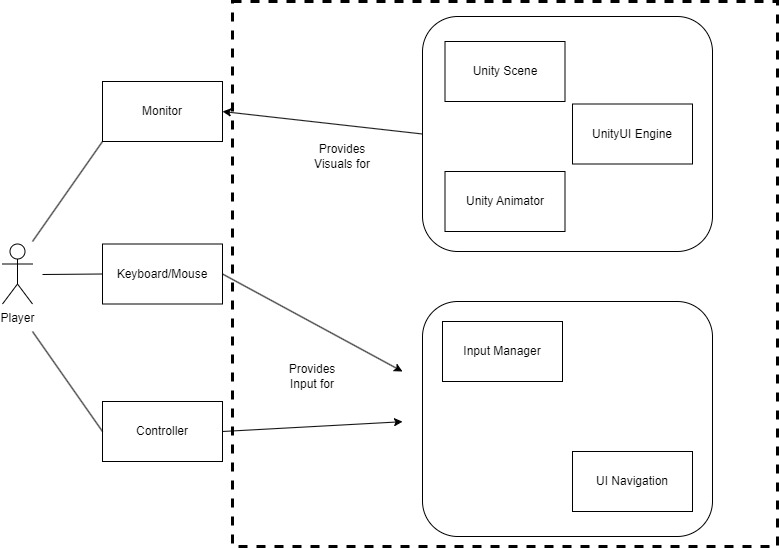
\includegraphics[width=0.5\linewidth]{images/physbound.jpg}
    \caption{Physical Boundaries}
    \label{phy_boundaries}
\end{figure}

\subsubsection{Logical}
%150 words minimum
% Describe the Logical System Boundaries.
The logical system boundary defines a scope of functions and actions and how they relate to each other. This is often represented in a diagram that has the various systems and functions and how they connect from front-end to back-end. The outside of the box represents the front-end and the back-end which in this case is the user and their machine and the back end is the database manager. The inside of the diagram represents various libraries and systems that help the front-end and back-end communicate and perform many different actions. Additionally, the inside also includes annotation labels to show how exactly different systems and/or actions connect. To explain the diagram above, we have a user who wants to send their user account and their game state data to the database where the admin can modify the data. Moreover, we have the player using the player and input manager classes to influence game state data being sent to the database.

\begin{figure}[ht!]
    \centering
    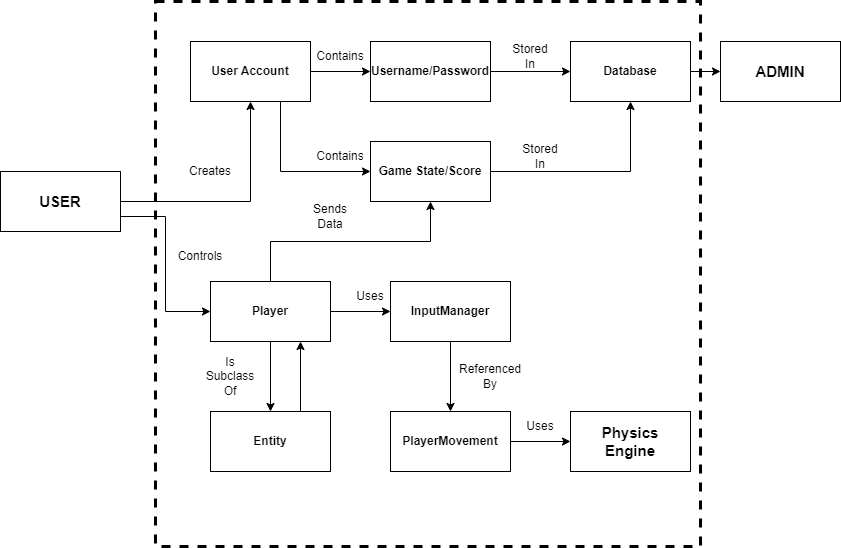
\includegraphics[width=0.5\linewidth]{images/logbound.png}
    \caption{Logical Boundaries}
    \label{log_boundaries}
\end{figure}

%---------------------------End System Boundaries------------------------------

% No text here.

%---------------------------Wireframes and Storyboard----------------------------------
\subsection{Wireframes and Storyboard}
%250 words minimum
% Use wireframes to create scenes and images of the user interface.  Connect the wireframes to show progression through the product to create a storyboard.  Describe the wireframes and storyboard.
Text goes here.

%uncomment the section below when you're ready to insert an image
%\begin{figure}[h!]
%    \centering
%    \includegraphics[width=0.5\textwidth]{images/picture_of_storyboard.png}
%    \caption{Description of the image here.}
%    \label{storyboard}
%\end{figure}

%---------------------------End Wireframes and Storyboard----------------------------------

% No text here.

%---------------------------Unified Modeling Language----------------------------------
\subsection{UML}

\subsubsection{Class Diagrams}
%At least one for each design pattern category.   
%Each class diagram should include the following:
%	Title for each Class Diagram
%	Description of how and why each class is used
%	Mapping to source code (in the Appendix, specific files and line numbers) of where it’s used.
For the Creational Object Oriented Design Pattern our project will be implementing the Factory pattern. The factory pattern provides a generic interface for creating objects and upon creation attributes are assigned to the generated object. In this project the Factory pattern will be used to solve the problem of creating multiple types of non-player character enemies by basing multiple NPC enemy classes on one main enemy interface. This design pattern is applicable because each enemy NPC will have differing health and damage amounts as well as different skins.

The Behavioral Object Oriented Design Pattern this project will apply is the state design pattern. The state pattern diagram allows an object to change the behavior based on state changes. This diagram covers the states of an enemy NPC which includes the Patrol, Attack, Damaged, and Dead states. This allows us to implement behaviors as a collection of self-contained components and will cause a reduction in condition code blocks in the project. This pattern is applicable to this class because enemy NPCs have different behavior states which can be easily encapsulated and organized via this design pattern.

The Structural Object Oriented Design Pattern this project will implement is the Decorator design pattern. The decorator design pattern is used to attach additional functionalities/responsibilities to an object dynamically - allowing for classes to be open for extension but closed for modification. In the project, the decorator pattern is applied to health orb power-ups that the player character can collect. The health orbs have different skins and heal the player for different amounts based on which variant is collected. This pattern is applicable as it allows for the health orb interface to be dynamically applied to a variety of health-orb powerups.


%uncomment the section below when you're ready to insert an image
\begin{figure}[ht!]
    \centering
    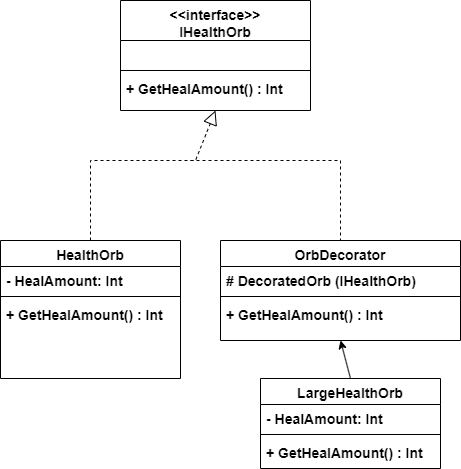
\includegraphics[width=0.5\linewidth]{images/oo/decorator.png}
    \caption{Decorator Diagram}
    \label{decorator_diagram}
\end{figure}

\begin{figure}[ht!]
    \centering
    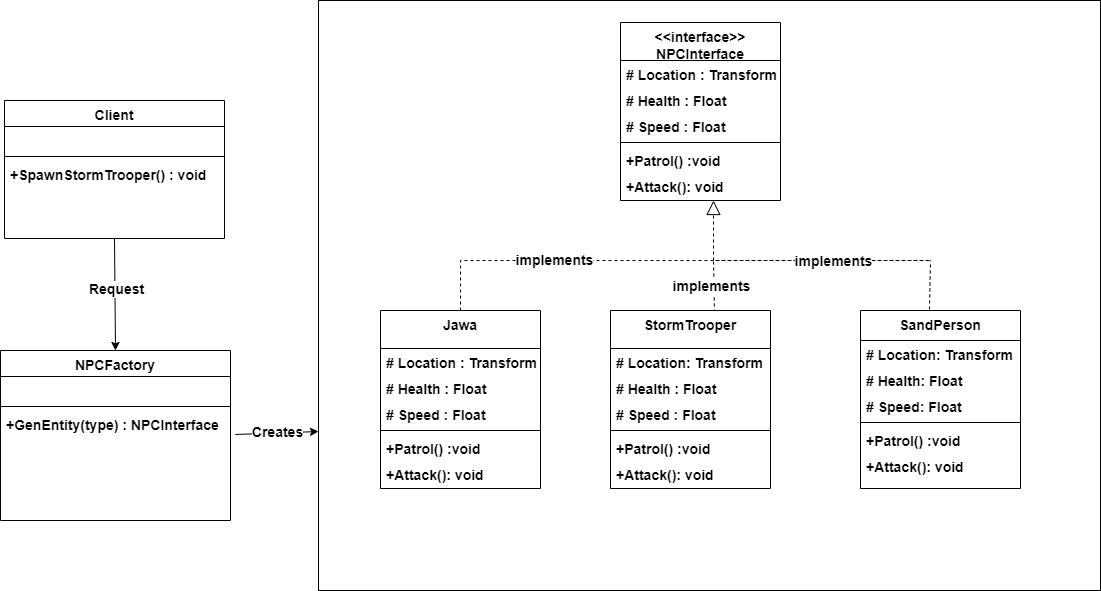
\includegraphics[width=0.5\linewidth]{images/oo/factory.png}
    \caption{Factory Diagram}
    \label{fac_diag}
\end{figure}

\begin{figure}[ht!]
    \centering
    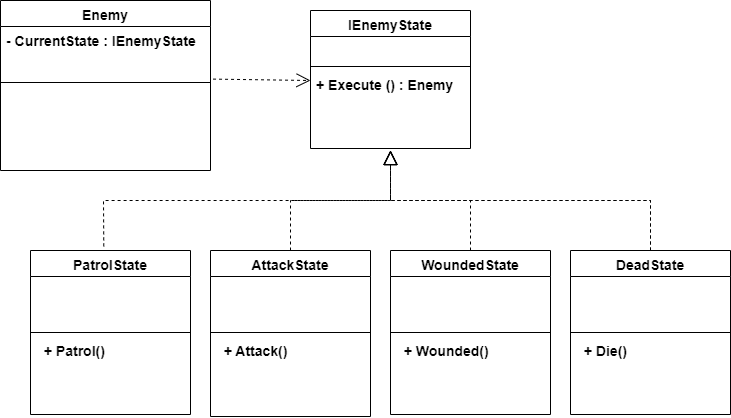
\includegraphics[width=0.5\linewidth]{images/oo/stateood.png}
    \caption{Model of EnemyStates}
    \label{enem_diag}
\end{figure}



\subsubsection{Use Case Diagrams}
%Enough to cover all technical functional requirements.
%Each Use Case Diagram should include the following:
%	Title for each Use Case Diagram
%	A description of information given in the diagram.
%	Mapping to source code (in the Appendix, specific files and line numbers) of where it’s used.
This use case diagram maps the higher level functionalities of the game, such as loading, saving, user input, and the user accounts functionality. This diagram will be really beneficial to us when we start breaking out issues into smaller tasks, and will likely serve as the foundation for our "epics," or overarching themes of an issue set. 

%uncomment the section below when you're ready to insert an image
\begin{figure}[ht!]
    \centering
    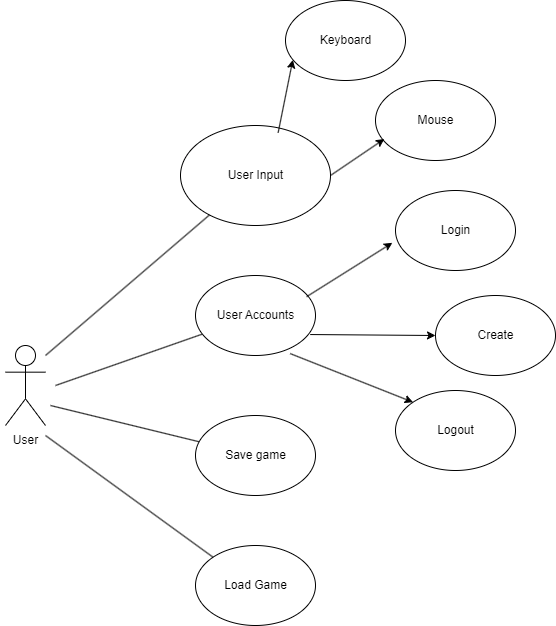
\includegraphics[width=0.5\linewidth]{images/usecase.png}
    \caption{Use case diagram}
    \label{use_case_scenario}
\end{figure}


\subsubsection{Use Case Scenarios Developed from Use Case Diagrams (Primary, Secondary)}
%Should include at least one primary and zero to many secondary scenarios
%Each Use Case Scenario should include the following:
%	Title for each Use Case Scenario
%	A short description of the information given in the scenario.
%	Mapping to source code (in the Appendix, specific files and line numbers) of where it’s used

\subsubsection{Use Case Scenario 1 (Based On 1st Use Case Diagram)}

ACTORS:
USER
COLLISION HANDLER

GOAL:
To detect collisions between different game objects that either player-owned or enemy entity game objects

SYSTEMS:
PHYSICS ENGINE
ENTITY TRANSFORM
COLLIDER

This scenario depicts how the user will interact with the physics engine in order to detect collectable items or enemies. This can be further applied to other objects like boost pads and hitbox detection for the speeder level.


\begin{figure}
    \centering
    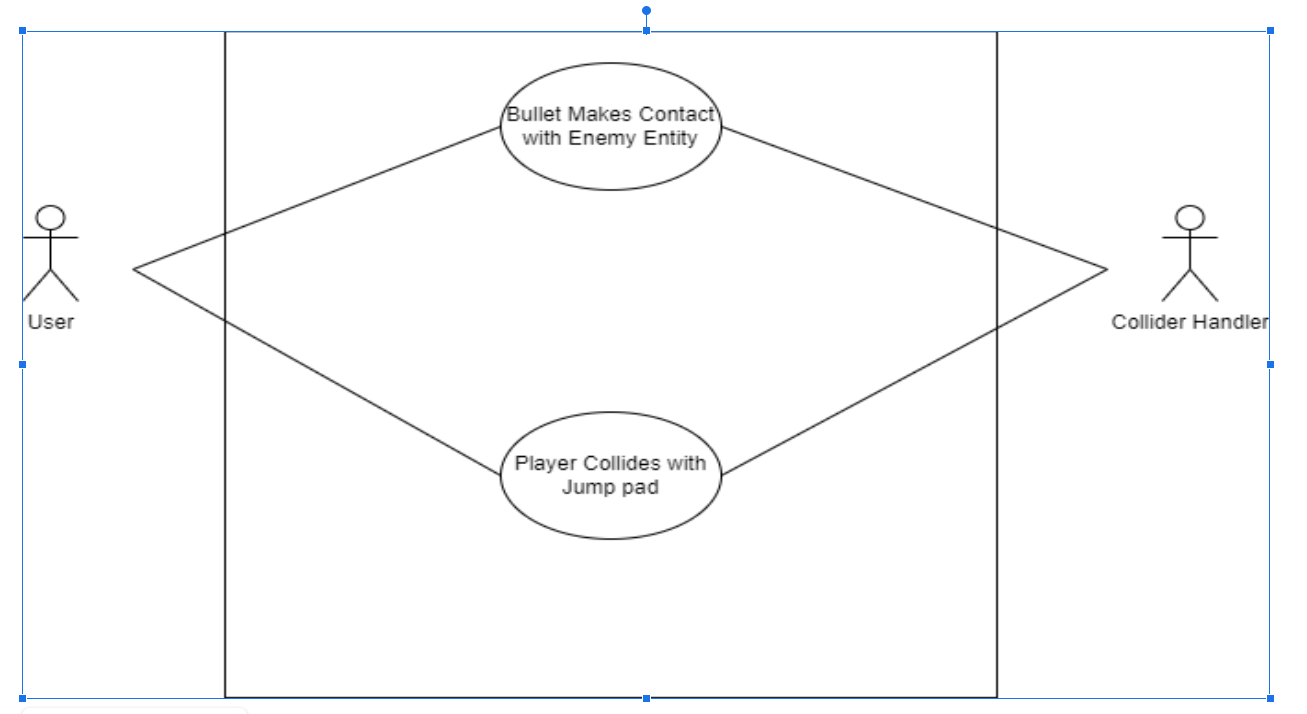
\includegraphics[width=0.5\linewidth]{firstuse.png}
    \caption{This use case diagram shows the relationship between the User actor and the collision handler. The actor will do actions such as doing damage to an enemy or using a jump pad which all use colliders and the collision handler will manage and send data back to the user.}
    \label{firstuse}
\end{figure}

\subsubsection{Use Case Scenario 2 (Based On 2ND Use Case Diagram)}

ACTORS:
GAMEMANAGER
ENTITY CLASS

GOAL:
To Allow the game manager to handle the spawning and despawning of entity objects through the entity class

SYSTEMS:
UNITY CLASS SYSTEM
ENTITY TRANSFORM

The scenario depicts the interaction  between the entity class and the game manager. The game manager will handle any level specific interactions like spawning and collectable placement.


\begin{figure}
    \centering
    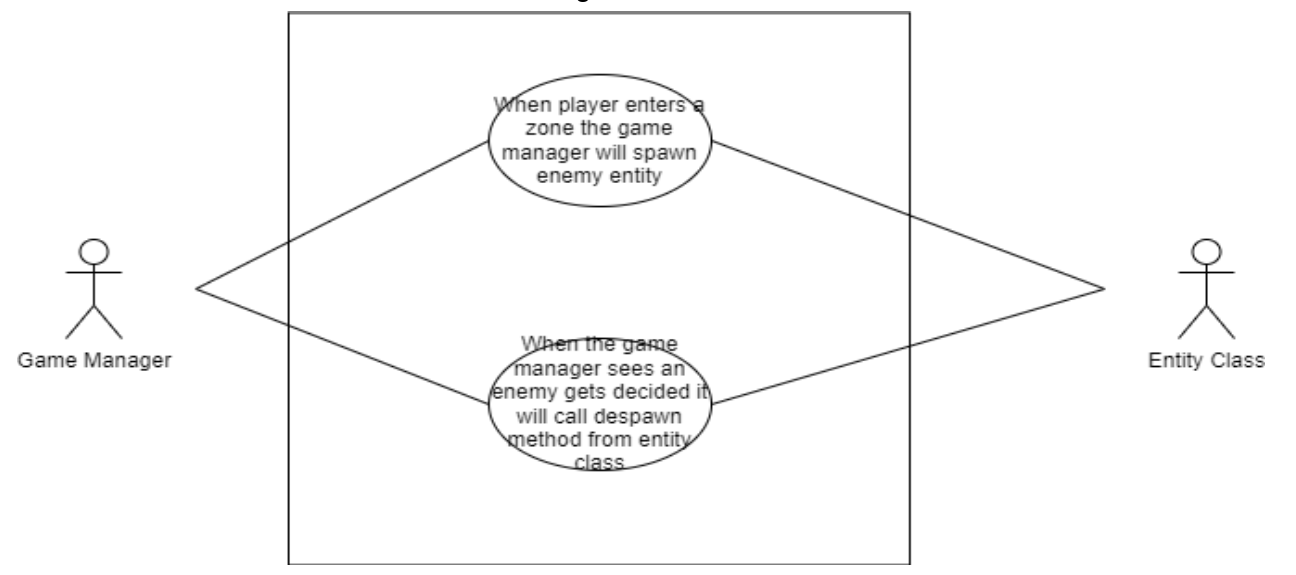
\includegraphics[width=0.5\linewidth]{seconduse.png}
    \caption{In this use case, we see the game manager as an actor and how it interacts with the entity class. The game manager when an event like an enemy dying or the player enters a zone will call functions from the entity class to spawn or despawn enemies.}
    \label{seconduse}
\end{figure}

\subsubsection{Sequence Diagrams}
%Each diagram should include all actors/resources to cover one Use Case Scenario.
%	Each Sequence Diagram should include the following:
%	Title for each Sequence Diagram
%	A short description of the information given in the diagram.
%	Mapping to source code (in the Appendix, specific files and line numbers) of where it’s used
The diagram above describes how we intend on implementing our authentication flow. We recognize that there may be additional steps necessary as we move down the line, but it is pretty straightforward. User will click the login button, which will take them to the login screen. Another way to do this is to just load the login screen first thing to the user, but I digress. After the user fills out the form, then the form is validated. Once we do this, we will compare the password to the one that is stored in the database and return a response to the user. Once the user is logged in, they will then be able to go to the main menu.

%uncomment the section below when you're ready to insert an image
\begin{figure}[ht!]
    \centering
    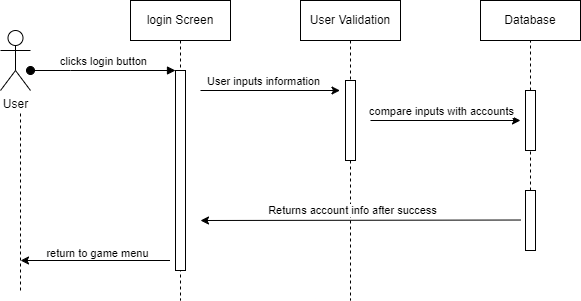
\includegraphics[width=0.5\linewidth]{images/sequence.png}
    \caption{Auth Flow Sequence Diagram}
    \label{auth_flow_diagram}
\end{figure}

\subsubsection{State Diagrams}
%Each diagram should identify the object/resource/asset (in the title of the diagram) and display all states and actions/events that create state changes.
%	Each State Diagram should include the following:
%	Title for each State Diagram
%	A short description of the information given in the diagram
%	Mapping to source code (in the Appendix, specific files and line numbers) of where it’s used
This diagram describes how the user will press certain buttons to control their characters. It is a pretty straightforward diagram, and most modern games will follow a similar style of implementation. The only thing that could be improved is that instead of giving a hardcoded key value combination, it could be an enum instead. This shows that we are thinking ahead to user control customization.

\begin{figure}[ht!]
    \centering
    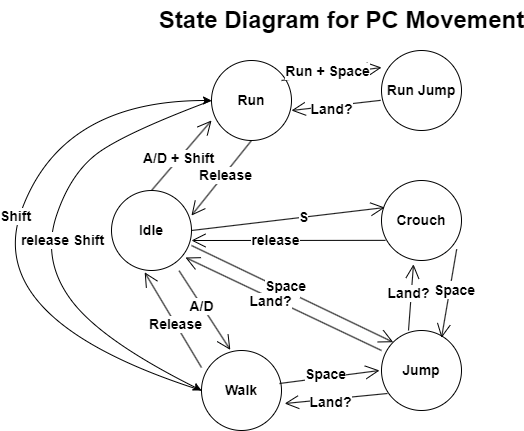
\includegraphics[width=0.5\linewidth]{images/oo/state.png}
    \caption{State Diagram for PC Movement}
    \label{class_diagram}
\end{figure}

\subsubsection{Component Diagrams}
%Single diagram that defines component APIs and communication pathways for all software and dependencies used in the product.
%	The Component Diagram should include the following:
%	Title for the Component Diagram
%	A description of the information given in the diagram
%	Protocols used for each communication pathway
%	Mapping to all source code and dependency software (in the Appendix, specific files)

This component diagram represents how the data models will be broken up, and how they will communicate with the database as a whole. The web server will be responsible for handling the interactions between the models and the database.

\begin{figure}[ht!]
    \centering
    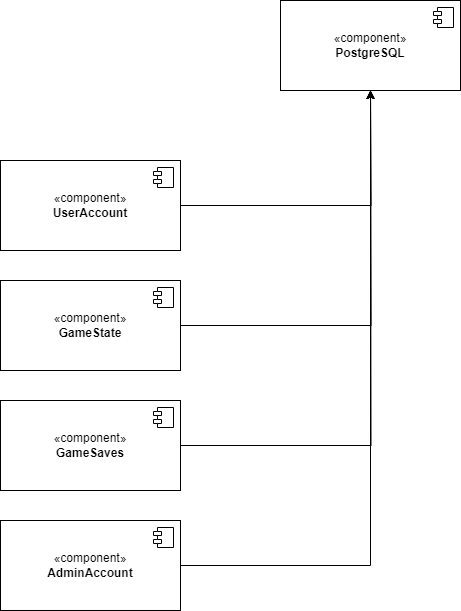
\includegraphics[width=0.5\linewidth]{images/component.png}
    \caption{High Level Database Model}
    \label{db_diagram}
\end{figure}

\subsubsection{Deployment Diagrams}
%Single diagram that defines the physical nodes, virtual nodes, and communication for all software related to the product.  Should be an extension of the Component Diagram.
%	The Deployment Diagram should include the following:
%	Title for the Deployment Diagram
%	A description of the information given in the diagram
%	Identify all physical and virtual nodes used for process execution
%	Identify all internal and external node communication

\begin{figure}
    \centering
    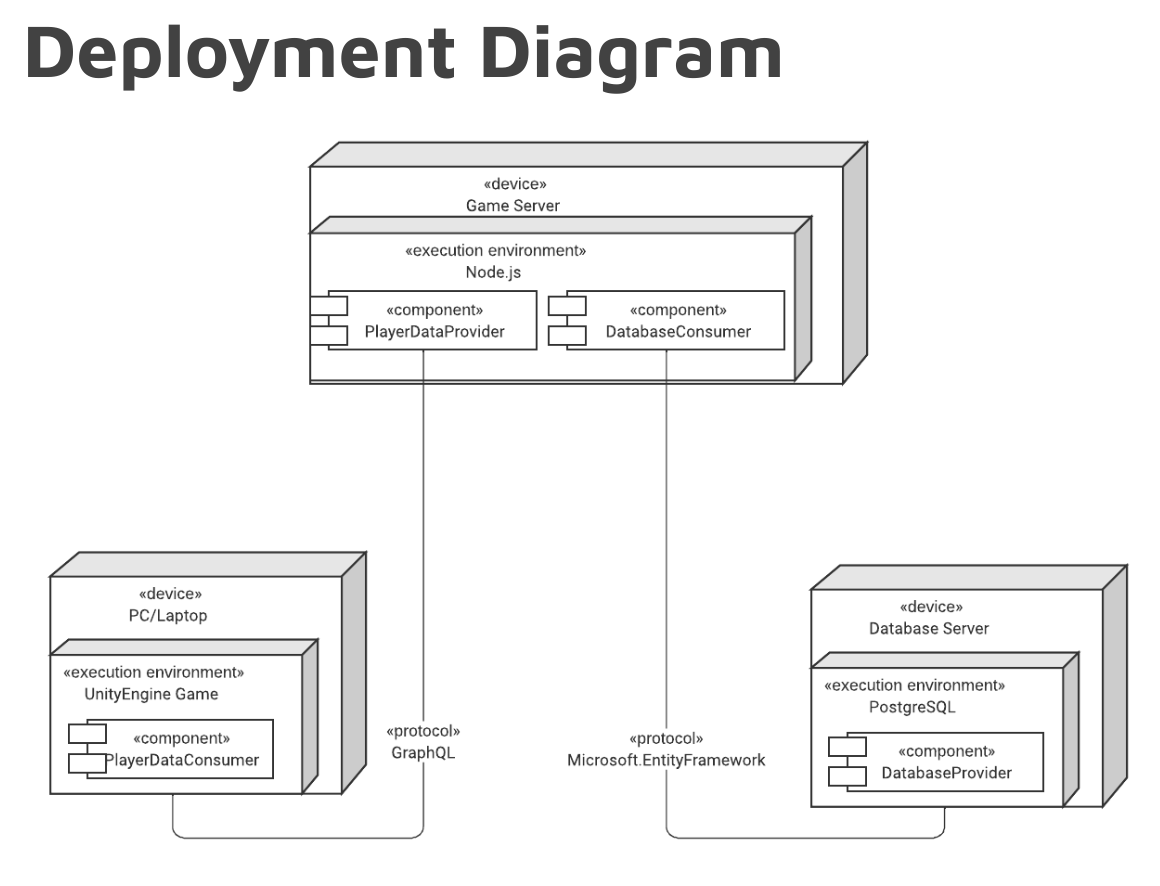
\includegraphics[width=0.5\linewidth]{images/deployment.png}
    \caption{Deployment Diagram}
    \label{deployment_diagram}
\end{figure}
%uncomment the section below when you're ready to insert an image
%\begin{figure}[h!]
%    \centering
%    \includegraphics[width=0.5\textwidth]{images/deployment_diagram.png}
%    \caption{Description of the image here.}
%    \label{deployment_diagram}
%\end{figure}

\subsection{Traceability Table}

\begin{figure}
    \centering
    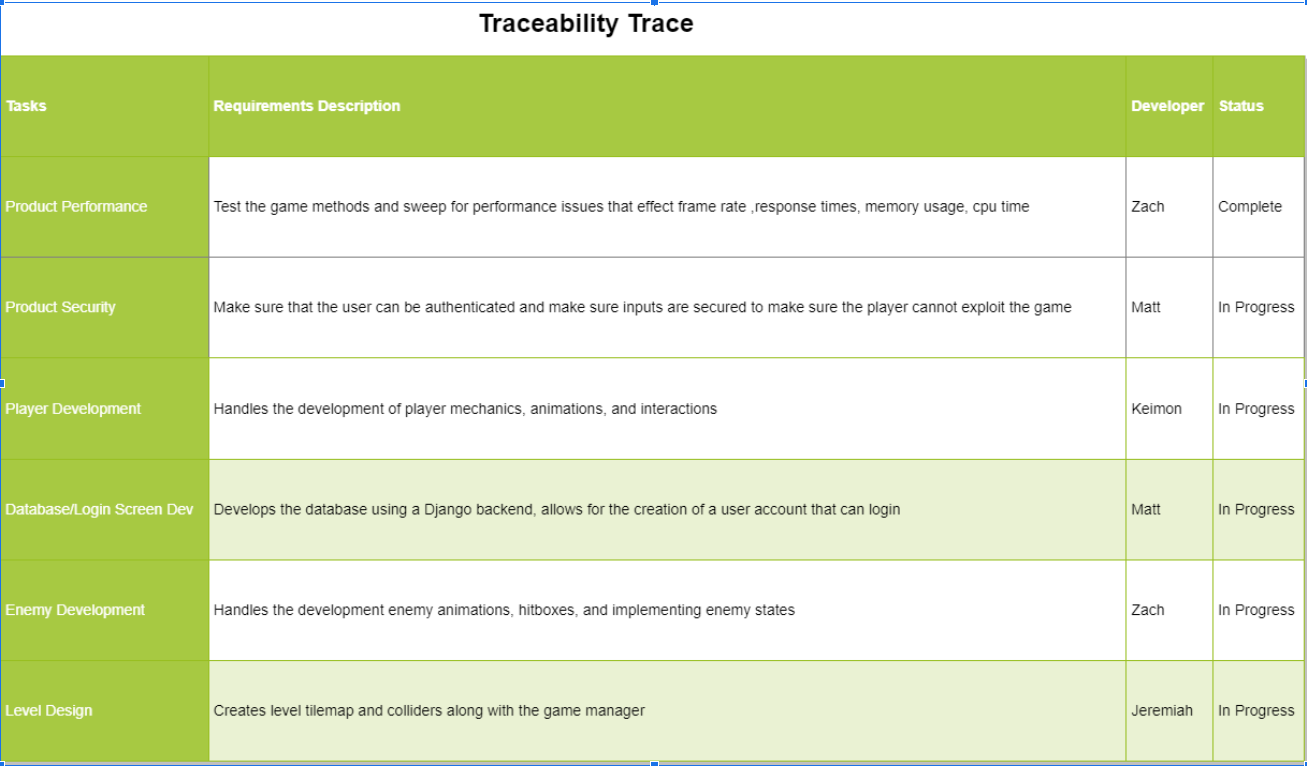
\includegraphics[width=0.5\linewidth]{images/trace.png}
    \caption{Traceability Table}
    \label{Traceability}
\end{figure}


%---------------------------End Unified Modeling Language----------------------------------

% No text here.

%---------------------------Version Control------------------------------------------------
\subsection{Version Control}
%200 words minimum
%Describe your group's approach to version control.  Include details on how and when you make commits to GitHub.  Explain version naming, branching, and integration approaches.

Our approach to version control is to use GitHub as our single source of truth for everything related to our project. This allows us to have control and consistency over our project management and codebase at all times. Moreover, it is also beneficial for keeping separate branches, thus always being able to have something presentable for the client. 

As far as when we make commits to GitHub, we haven't made too many commits other than to store files such as our organization.tex and technical.tex, but we plan to make commits to our GitHub anytime that we make changes to the codebase of our upcoming Unity project. The way we will be doing so will adopt a master <- develop <- feature hierarchy, in that all changes will be first made in a feature branch, and then merged into the develop branch. This is where we will QA new features and PRs. Once they have passed the QA and testing stage, we will merge into our main branch.

As far as keeping track of issues, we have decided to adopt the Epic <- User Story <- Feature / Bug model of issues. This allows us to make higher level goals (epics), break them into medium sized bodies of work (stories), and then break those up into bite size pieces of work (feature / bugs). This allows us more granular insight into how our project is moving along relative to the timeline of our sprints. 


%---------------------------End Version Control------------------------------------------------

% No text here.




%---------------------------End Data Dictionary------------------------------------------------


% No text here.

%---------------------------User Experience Details------------------------------------------------
\subsection{User Experience}

\subsubsection{Gameplay Diagram}
%150 words minimum
%Also called a controlled flow graph.  Insert an image of the gameplay diagram and describe the diagram in detail.
This section of the document will talk about a gameplay flowchart and describe it. As one can see in the diagram the base of the flowchart is that the player is moving through the level. We have multiple things that can appear. For instance if there is an enemy. If there is one they can shoot or avoid said enemy. Then they see if there is an obstacle or a gap in the platform. If it is a yes they jump over said obstacle or gap. If not they keep moving forward. There is also a part that says was an item picked up and if one was an effect is applied based on what the item was. If not the player gains nothing and keeps moving. And finally a check on if the player has died. If yes they restart the level if they have an extra life or they get a game over if they do not have an extra life. If they don't die they keep playing. 

\begin{figure}
    \centering
    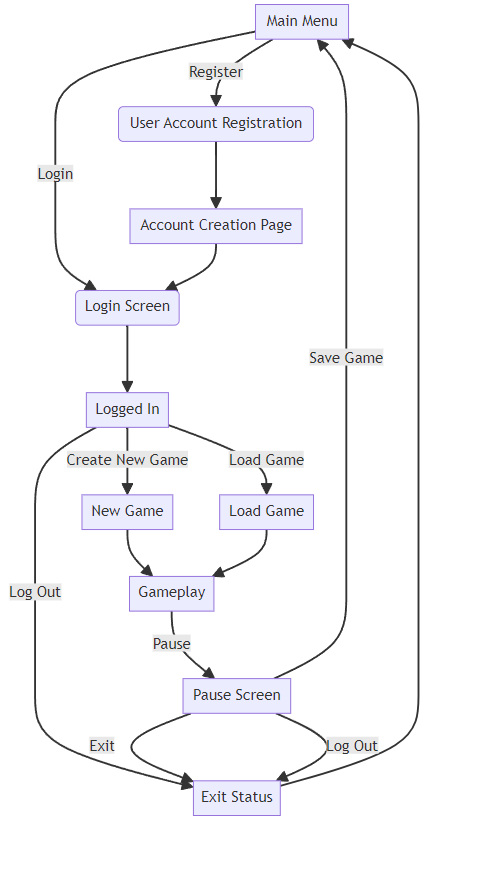
\includegraphics[width=0.5\linewidth]{images/gameplaydiagram.png}
    \caption{Gameplay Diagram}
    \label{gameplaydiagram}
\end{figure}

%uncomment the section below when you're ready to insert an image
%\begin{figure}[h!]
%    \centering
%    \includegraphics[width=0.5\textwidth]{images/gameplay_diagram.png}
%    \caption{Description of the image here.}
%    \label{gameplay_diagram}
%\end{figure}

\subsubsection{Gameplay Objectives}
%150 words minimum
%Should explain why someone should play your game. Should define the goals of your game.
This section will talk about the gameplay objectives, which will be about the goal that the player is striving for. As well as talking about why someone should play this game. To start off I would like to discuss why someone should play our game. I feel that people should play our game because it is a fun platformer that takes place in the Star Wars universe. In this game you play as the famous character Luke Skywalker as he attempts to save the galaxy. Another thing is that this story allows the player to play through the same story from the movies which allows the player to live through the story from a more interactive place.

The overall goal of the game is like that from the movies. You are trying to defeat Darth Vader and save the galaxy from the Empire. How you will do this is that you will have to dodge, fight, and avoid enemies of each level. Ultimately making it to the end of said level and moving on to the next. You will also have to traverse through dangerous spikes and other environmental dangers.


\subsubsection{User Skillset}
%150 words minimum
%Describe the abilities a user should have in order to interact with the software: Screen tapping, Memorization, Puzzle, solving, Strategy development, Quick reflexes 
This section will discuss the user skillset. This means this section will be about the necessary user abilities necessary to effectively play this game. One of the most important skills the player should have is that they will need to have quick reflexes. This game will have enemies attacking you as you try to platform. If you are unable to react quick enough you will get killed many times by the enemies. Another necessary skill the user should have is timing. The reason for this is that you will need to know when to hit the jump button to make it to another platform, as well as when it is okay to attack the enemy back as if you try and do it at the wrong time you will get hit by an enemy blaster. The player will also need to effectively use the keyboard as if they do not know where keys are or are not used to keyboard controls they might not be able to perform the required actions effectively.

\subsubsection{Gameplay mechanics}
%150 words minimum
%Thorough guide of the game rules: Turn-based, Random chances, Capturing/eliminating, Time-based, Team-based
This section will be about the game mechanics for this game. The mechanics that this game is based on are platformer mechanics and a bit of some run and gun. The platformer part comes from the fact that you are tasked with getting to the end of the level all the while you avoid terrain dangers and enemies. You will jump between different platforms and try your best to not fall off or be killed by the previously explained dangers. This is where a bit of the run and gun comes from. The player will have a weapon to defend yourself and beat the enemies as you traverse the level. The player will be able to shoot their blaster at the enemies and at some point will have a lightsaber to attack as well. As well as looking out for life orbs to heal the player after getting hurt by something or even getting an extra life. The overall package being that you will run, jump, crouch behind cover, shoot, slice with your lightsaber, and pick up helpful items to help you get through the game.

\subsubsection{Gameplay Items}
%150 words minimum
%This section of the GDD refers to smaller elements of the game, such as: Health/power-ups, Coins, Loot crates, Weapons/character upgrades, Etc. Changes gameplay elements as the player progresses through the game.
This section of the document will involve the gameplay items. This entails the smaller components of our game that will slightly change the flow of the game as it is played. The first gameplay item that will be discussed will be the small health orb. The small health orb will recover the player’s health by a small margin. This won’t be a whole lot of health but this will allow the player to survive a few more hits and help them out when they are in a pinch. An item that is like the first but better would be the large health orb as this item will greatly recover the players health. Meaning that they could be on the brink of death and after picking up a large health orb they are doing okay, and are now able to take a few more risks. Another item would be the extra life as this will allow the player to make a mistake and have another chance at completing the level before a game over takes place. 

\subsubsection{Gameplay Challenges}
%150 words minimum
%Description of game challenges as a player progresses. Identify how a player handles difficulties and ensures the player can obtain essential tools to continue progressing through the game.
This section will discuss the gameplay challenges of our game. This will entail the challenges a player is expected to face as well as how they are expected to get past said challenges. For the challenges that the player is going to come up against it will be against dangerous terrain and enemies. For the terrain it can be spikes, falling objects, and even bottomless falls. The player will be expected to learn the patterns for falling objects through some observation and thought out movement. We will also ensure that the placement of said objects are fair. For the spikes and bottomless pits the player will handle these through well placed jumps and observations. We will also ensure placement of these things are fair as well. For the enemies the player will have to deal with these by using their wits and the weapons they are supplied to deal with them. For instance the player can duck to evade a blaster or they can jump. Based on the environment will depend on what works better for the current instance as well. We will ensure that the enemies are well placed throughout the level. 

\subsubsection{Gameplay Menu Screens}
%150 words minimum and wireframes
%Game start menu screen, pause menu screen, game over screen
%Give wireframe/drawing/image for all menus in the game.
This section will go through the menu screens that will be seen in this game. The first screen that you will find when you enter the game will be the login/signup screen. These will be found on the left side of the screen as the star wars logo is shown on the right. After logging in you will see the main menu screen which will have your account on the upper left part of the screen and the high scores on the right. Under the account info you will find a load game, new game, settings, and controls button. Clicking the load game button will take you to a menu that will have all the loads that are owned by your account and each will have a resume button. The new game will just start the game and you will start to play. The settings function will take you to a menu that will allow you to change certain aspects of the game. The controls button will take you to a menu that will allow you to change your button layout and allow the player to change what button does what. While playing in the game if you press a certain button you will be taken to a pause menu which will allow the player to save the game, quit, or resume. Quitting will then take you back to the main menu screen.

\subsubsection{Gameplay Heads-Up Display}
%150 words minimum and wireframes
%Current Game information visually relayed to the player as a part of the game’s user interface.
%HUD features are generally static, on-screen so they remain visible during gameplay. Health/Lives, Time, Weapons/Ammo, Capabilities, Menus, Mini-Map, Score, etc.
This section will talk about the heads up display that will be in the game. This generally entails life bars, scores, and anything that is on the screen that the player uses to understand the current game state. For our game we will have three different displays, and these displays will be a life bar, a score, and extra life counter. These can be seen in the diagram but to explain a bit more in depth is that the life bar will be vertical and will be in the left upper corner. For the extra life counter we will put it in the right upper corner of the screen and it will display a small sprite of the player's character with a number beside it. This number will signify the amount of lives the player currently has left. For the score it will be placed in the bottom right of the screen and this will show the current score that the player has.

\subsubsection{Gameplay Art Style}
%100 words minimum
%describe the visual appearance of characters, objects, and other in-game elements. (Realistic, Cartoon, etc.)
In this section of the documentation the art style of the game will be the topic of discussion. The art style that was chosen for this game was the use of pixel art. This is an art style that reflects the older days of gaming but can still look very good when everything is well detailed. This means all in-game things will have a more cartoon look to it. Every character will have a decently detailed sprite using this pixel art. As well as the scenery and menus. The terrain and scenery will have one sprite and not change its look. The enemies and characters though will use multiple sprites so that all their actions can be well animated. For any cutscenes even though the pixel art style is being used it will have a cartoon look to it but characters will look close to what is seen in the movies.



\subsubsection{Gameplay Audio}
%150 words minimum
%Description of all game audio: Character sound/voices, Ambient world sounds, Background music, etc.
This section of the document will talk about the gameplay audio. This will entail any sounds that the player will hear while playing the game. First thing will be damage noises and death sounds. These will be played when the player is hit or when an enemy is hit and these will be unique. The same goes for the death sounds as both the player and enemies will have a unique death sound. These will be auditory cues to help the player identify if an enemy has died and who has taken a hit. Another important audio feature that will be included will be the background music. The plan for this is to be engaging but not overbearing. As its name implies it is for background noise. This music will be something that relates to the Star Wars franchise. Basically it will be music that is from Star Wars. Another piece of audio that will be played will be a sound that will go over top of the player's gun. Whenever the player shoots it will play a quick sound. Finally item pick ups will have a confirmation jingle. Basically on pick they will play a sound that will inform the player it was successfully picked up.



%---------------------------End User Experience Details------------------------------------------------

% No text here.


%---------------------------End Modeling and Design Section----------------------------------


% No text here.


%---------------------------Non-Functional Product Details Section---------------------------
\section{Non-Functional Product Details}

%---------------------------Product Security-------------------------------------------------

\subsection{Product Security}

\subsubsection{Approach to Security in all Process Steps}
%250 words minimum
%Describe how your team modified the original technical document to address security issues in the Requirements, Modeling and Design, and Implementation sections.

When considering security in a game, there are a couple of ways to do so. First, what can the client change about their game? Can they make their player move in ways they should not be able to? Can they glitch through parts of the level? Can they cheat and get an unrealistic high score? These are client side risks, that are generally a concern in games that are singleplayer. Yes, this game is single player, but basically everything other than the actual gameplay itself must be authenticated on the Django game server.

When a user logs in, the game will store their credentials (JWT key) for future use. Whenever a user wants to perform any action such as changing their settings, saving or loading a level, or logging in, they MUST provide credentials or the Django server will decline the request. 

We perform our API requests using the System.Net.Http class provided by C\#. This ensures that our requests are done via HTTPS, which will automatically encrypt any data that is sent over it. Finally, Django also has safeguards in place for common attacks such as CSRF forging, XSS, and more. Choosing Django has allowed us to already have security features such as securely storing user passwords via hashing. Moreover, it allows us to extend these default user attributes and add some of our own. This helps by making it easier for us to implement user data, and it does so more securely as we are not trying to implement hashing ourselves. Doing this removes a possible avenue for attack.

Overall, we are really happy with the security of our product. I am sure there are plenty more things we should be doing, but for now this is a good start.


\subsubsection{Security Threat Model}
%200 words minimum and Security Threat Model
%Create and add a Security Threat Model, related to the Deployment Diagram, that identifies trust boundaries and potential security risks

Our security threat model has three areas: 1. the User, 2. the Game server, 3. the database. The boundary between the user and the game server is one that can only be accessed with user credentials. Even then, they only have access to modify their own data, no one else. The boundary between the game server and the database is a more touchy one especially if we were directly interacting with the database instead of using a web framework like Django. This removes risks such as SQL injection because we never make a SQL call to the database, we only interact with the data via models in Python. 

The biggest risk would be if somehow a Django secret key got leaked after production, and people were able to spoof API requests to a phony Django server. However, this is not easily done, and can be easily mitigated by using environment variables for any secret keys. This way, your repository never stores any sensitive data.

\begin{figure}
    \centering
    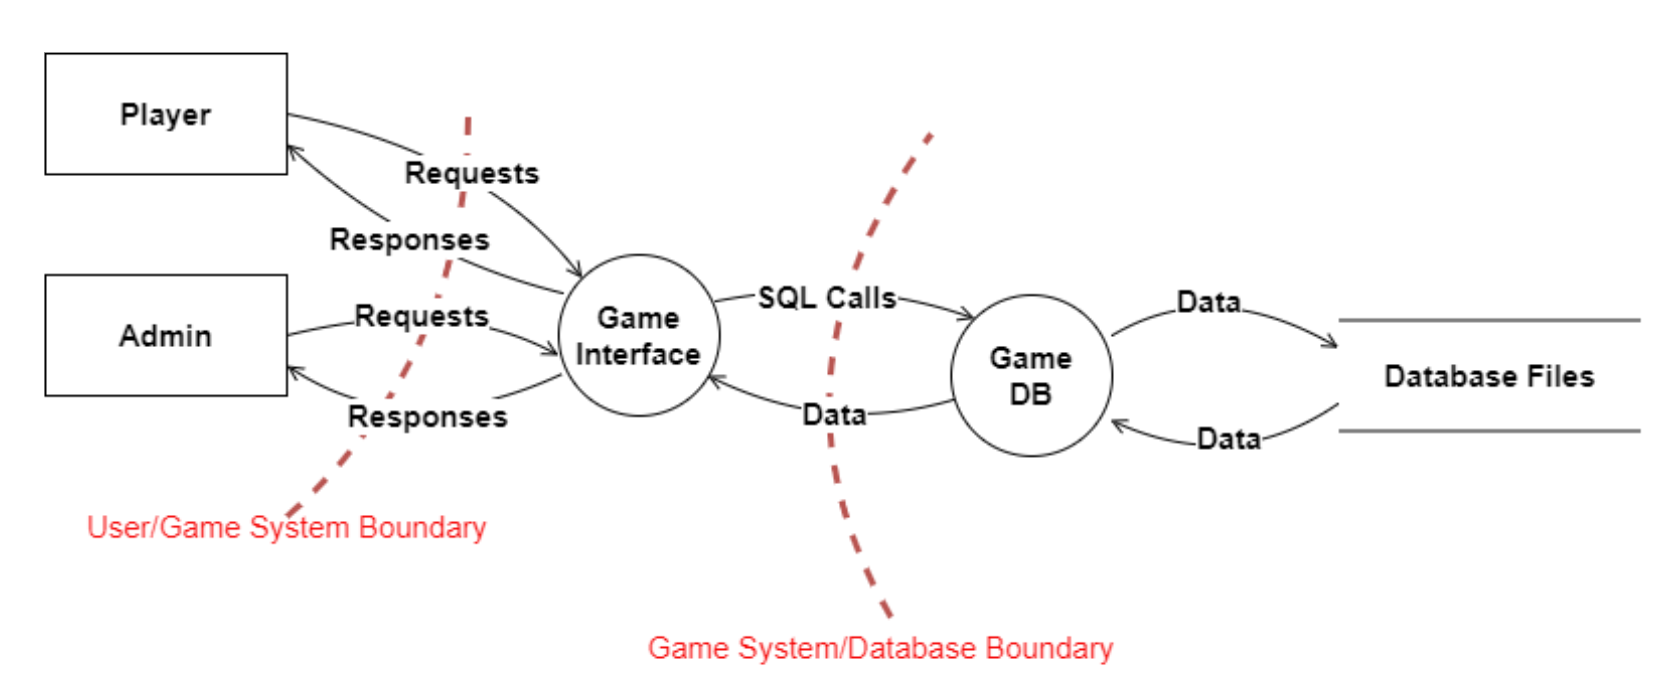
\includegraphics[width=0.5\linewidth]{images/threat.png}
    \caption{Enter Caption}
    \label{fig:Security-threat}
\end{figure}

\subsubsection{Security Levels}
%250 words minimum
%Describe the different security levels for general users and administrators.  Also describe the authentication/authorization techniques for users of the software product.

In security, you should follow the practice of give NO permissions by default, and give only the ones that are required. So, we are going to follow this rule.
Default users will not even have access to the Django admin panel what so ever. They can only use the UI provided in the game to update their data such as settings, saves, user data, and more. 

In contrast, the admin user will have full destructive access over the database and app itself. The admin will have access to add / remove high scores, add / remove user saves, delete users, and everything an admin should have access to. If we were handing this off to an end user, we would likely not give them full access, but just the permissions they would need. This removes the risk of having a careless manager who leaks their admin credentials, and minimizes the would be damages. 

The way that a user is authenticated is by sending a POST request to cs360.irizarry.dev/accounts/login and if the login is successful, it will return a user object with the user credentials in it. The credentials are stored and then will be used in subsequent requests that require authentication. The app also supports /accounts/register.

%---------------------------End Product Security-------------------------------------------------

% No text here.

%---------------------------Product Performance-------------------------------------------------

\subsection{Product Performance}


\subsubsection{Product Performance Requirements}
%200 words minimum and list of performance non-functional requirements.
%Define and justify performance requirements.  These should be added to the list of non-functional requirements.
The performance requirements should be set to ensure a smooth and satisfying user experience. If the performance of a product is not adequate for a consistent and fluid user experience then users will be unsatisfied and will not want to utilize the software. 

Our target hardware is one of the team member’s laptops, which has an AMD Ryzen 7 processor with an integrated graphics card and 16GB RAM, this should be more than sufficient for this project. For this product, we will track frames per second (FPS), CPU time, memory usage, duration of method calls, and time elapsed on database calls. The aim is to maintain a high frame rate (FPS) at equal or greater than 60 frames per second. The target CPU time for gameplay is less than 16ms. It should be acknowledged that at the lower end of the spectrum relative standard deviation is a faulty metric because even a change of a couple ms can drastically increase this measurement; as such this measurement will only be considered as performance approaches the minimum requirements. It is essential that our database operations be quick to ensure a positive user experience; therefore, database operations such as user authentication and save/load game states should take a maximum of 2 seconds. Finally, the game should be very responsive to user inputs and should respond to user input within 50 milliseconds, for this method calls will be observed for their duration. As development continues requirements will be set to set limits on scene switching times, throughput, load testing, and stress testing.

By keeping defining the performance requirements before development, it helps ensure that the development process will result in a good product. Additionally, it is important to measure and track these requirements throughout development so that mistakes or low performance can be caught and remediated. 


\subsubsection{Measurable Performance Objectives}
%200 minimum words and list of objectives.
%Measurable Performance Objectives should be stated in this section that relate to the performance requirements.
To adequately meet product performance requirements it is essential that performance be measured throughout development. Measuring performance allows the team to monitor defined metrics and find bottlenecks and correct them. To track the gameplay metrics of FPS, CPU Time, and memory usage the team created an empty game object named ‘pTest’ and placed it in the scene. A script was then attached to ‘pTest’ which outputs the CPU time, FPS, and memory usage to a .log file every frame. As stated above the goals of 60 FPS, a maximum of 16 ms CPU time, and less than 2 GB memory usage have been set to ensure a smooth user experience. The goal for CPU time is 16ms or less, but the target is really consistent performance meaning the game should avoid major spikes in CPU usage. Relative standard deviation of CPU time should be kept under 5-10\%, particularly as CPU time approaches 16ms. Currently it is not possible to implement testing for scene loading time because the game currently has only one scene implemented and no menus to load from. Stress and load testing are also not very feasible given our limited implementation, but these requirements will be set and tested as development progress is made.

\subsubsection{Application Workload}
%250 words minimum
%Application Workload information should be gathered and visualized in this section.  This generally requires historical data on how the software product is being used.  For example, users generally spend 10% of the time interacting with menus, 80% of the time interacting with main features, 5% of the time saving work, etc.  These workloads should not be assumptions or guesses.  Timers need to be created for all major UI features of the product to generate reliable application workload analysis.
Application workload analysis is important so developers can track how users are interacting with the product. This can showcase potential difficulties in the menu system, allowing the team to modify the user interface to be more straightforward. Additionally, this type of testing will highlight the most used parts of the game (perhaps monitoring the top scores) which would help the team allocate resources to enhance the overall user experience.
At this time in the development process, the user interface is non-functional and has not yet been implemented in the design. Therefore, we do not have direct historical data to demonstrate accurate workload measurements and percentages. To accomplish this in the future timers will be created on all major UI features, which will allow the team to monitor time spent on each feature. Some of these timers will include but are not limited to: main menu timer, gameplay timer, scoreboard timer, save/load game timer, login timer. In addition to timers, it would be useful to add even trackers to record specific actions, such as the number of times menus are accessed, how often a game is saved/loaded, number of times the game is paused and resumed. In a real world scenario, it would also be useful to deploy surveys and feedback forms during the testing phases, which would provide valuable feedback and insights on UI and workload analysis. A hypothetical workload might look like 10\% of time spent in main menu interactions, 80\% of time playing games, 3\% of time saving and loading the game, 2\% of time logging in, and 5\% of time looking at highscore menus. These hypothetical numbers can serve as a loose goal for the future. 

\subsubsection{Hardware and Software Bottlenecks}
%250 words minimum
%Hardware and Software Bottlenecks should be identified and discussed in this section, with test cases to justlify.
Hardware and software bottlenecks are parts of a system where performance capacity is significantly lower than other points, creating a gap in capacity which can affect the overall efficiency of the system. It is essential to identify and address these bottlenecks to prevent system failures, delays, user dissatisfaction, and increased costs. This is a key portion of system optimization and is essential to monitor in order to create and maintain a responsive product.

Major potential hardware bottlenecks include reading data from the disk, shortage of memory, moving data from memory to CPU, and network capacity. In terms of our project this would look like database read and writes for save games, highscores, and logins. Additionally, because the team has opted for a live Django server to host the database, network connectivity could be a major bottleneck as well. 

Possible software bottlenecks include poorly written algorithms that do not scale well with the scope of the program. This is a risk we are currently monitoring via method call timers and code reviews. The performance testing that is being conducted would also highlight potential bottlenecks. Overall, the largest performance bottleneck our project may face is the Unity Engine because Star Wars SMS is a very light 2D platformer that will be very light performance wise. 

So far, the product is well within the defined requirements and there are no glaring bottlenecks or issues that are going to cause performance issues as of yet. This will be an area we will continue to monitor via testing to see if anything arises.


\subsubsection{Synthetic Performance Benchmarks}
%250 words minimum
%Synthetic Performance Benchmark test cases should be developed and executed on target hardware.  Results should be visualized and discussed in terms of the required target hardware details. (File I/O, CPU, Database).  Sysbench
Synthetic performance benchmark testing is important for developing software for a target system because it allows developers to see how well a system can handle demands that its application might pose. The benchmark tests were performed on a device that is within the target hardware specifications, which was a laptop with AMD Ryzen 7 5825U processor with Radeon Graphics (2.00 GHz), and 16.0 GB RAM.

The CPU performance tests were run using the following line ‘sysbench cpu --threads=X --cpu-max-prime=15000 run’ using thread counts of 1, 2, 4, 8, 16, 32, and 64. Each thread count was run five times on the target machine to demonstrate an average metric which can be used to establish a trend in CPU performance.The execution time increases linearly with the increasing number of threads, this is expected because more time is dedicated by the CPU to manage thread management and switching. The total number of events increases drastically as the number of threads increases from 1 to 16, suggesting the CPU is able to handle much more work as more threads are added up to a certain point. From 16 threads on the average elapsed time increases but the number of events does not, meaning that the overhead cost of managing that number of threads outweighs the added performance (which in this case is not much).

The file input/output tests were run using this line ‘sysbench fileio --file-total-size=X --file-test-mode=rndrw –threads=8 run’. These tests were run using a variety of different file sizes ranging from 512 MB to 32 GB. Each test was run a total of five times to establish a trend in system performance. The execution time of each file size was fairly constant, only increasing significantly for larger file sizes. The throughput of read and writes remains fairly constant across file sizes, except for the 32GB file size, which shows a higher throughput for both read and write.

The results of the synthetic benchmark tests allow the team to see potential bottlenecks in system performance and potential areas of concern. In the case of this software product and the target software, we determine that our hardware performance will not be an issue in the performance of our product. In the future it would be useful to implement testing on the database using sysbench or another similar performance software to establish boundaries in the database performance as well. 

\begin{figure}
    \centering
    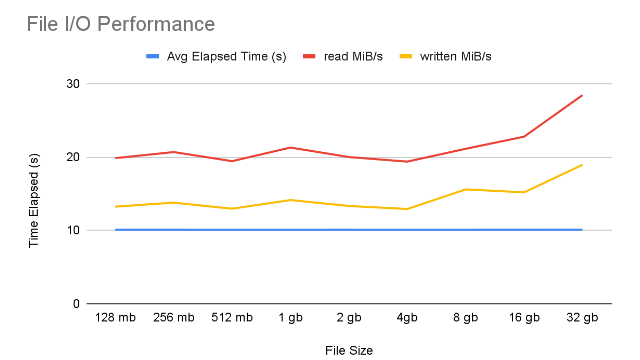
\includegraphics[width=0.5\linewidth]{fileioperf.png}
    \caption{FILE IO Perf}
    \label{perf}
\end{figure}

\begin{figure}
    \centering
    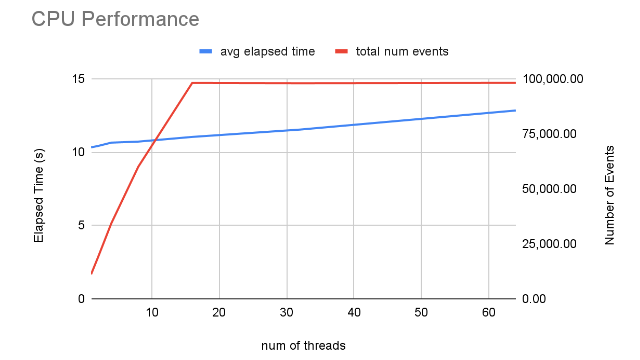
\includegraphics[width=0.5\linewidth]{cpuperf.png}
    \caption{CPU Perf}
    \label{cpuperf}
\end{figure}

\subsubsection{Performance Tests}
%250 words minimum and test case description with results
%Performance Test Cases should be given in this section.  Test Cases should be executed and results should be visualized (Images, Graphs, etc.)
%examples of performance tests include, but not limited to: Load testing (expected and peak loads, exceeding peak loads), Stress testing, throughput testing, function call timers, compatability testing, fault tolerance testing, etc.

Performance testing is important in game development to ensure a smooth user experience. Gameplay should be monitored for consistent performance, without lag or crashes, which is essential for user satisfaction. So far, FPS, CPU Time, Memory usage, and method call duration are what have been implemented and monitored. These metrics will allow for monitoring of basic game performance in the scene we have implemented and would allow us to detect any hindrances in performance if there were any. Method call monitoring highlights possible inefficient code and helps give the team possible sections of code that need to be refactored. The method calls that have been implemented so far perform within our expectations and do not slow the game in any capacity. Additional areas of testing include throughput testing, stress testing, and load testing which could be designed and implemented in the future to determine the performance resilience of the game. Game scene transitions as well as database read/write speeds are planned on being monitored once those features are implemented. In previous sections, the methodology for our performance testing was discussed in detail, as well as future plans to implement said tests. So far the performance of the game exceeds our performance requirements and does not showcase any areas for improvements or any bottlenecks. These areas will continue to be monitored to showcase any issues that may arise.
\subsubsection{Method Time Tests}
\begin{figure}
    \centering
    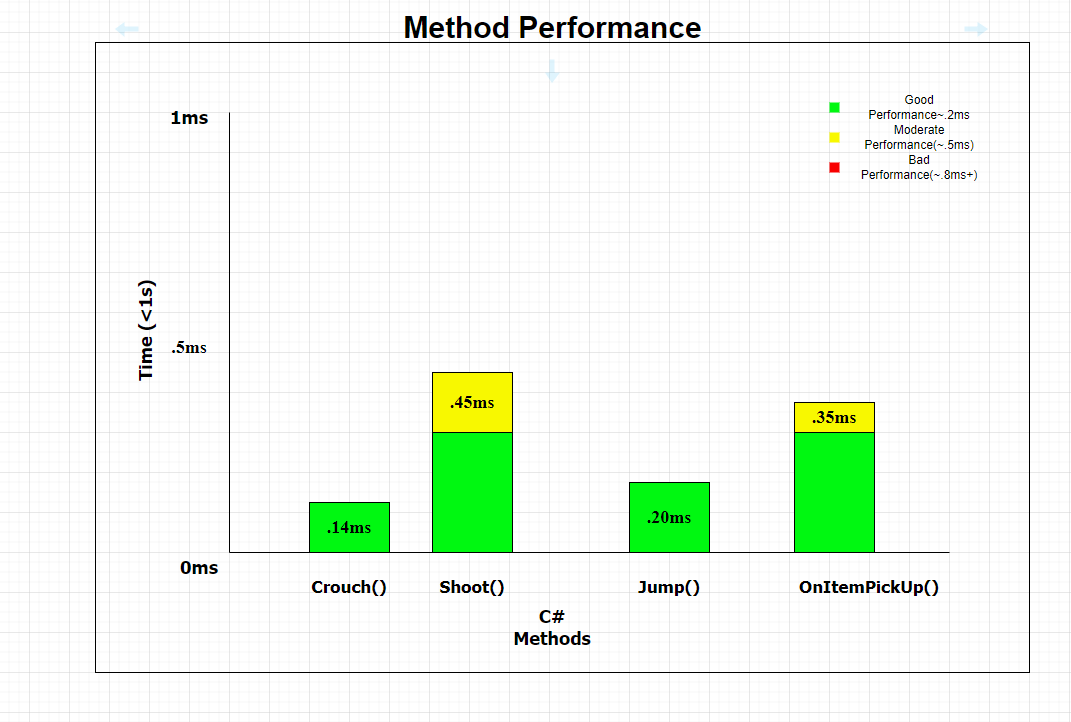
\includegraphics[width=0.5\linewidth]{methodtime.png}
    \caption{Method Time Graph}
    \label{fig:enter-label}
\end{figure}
In order to perform a performance test of the in-game c sharp functions, a script that would allow for the functions start and finish times to be exported to a log file document with the ability to check how many milliseconds has passed since the native Unity console log does not check for milliseconds. We also did this so that we could store the log as unity logs resets every replay and we would like to archive data for a longer time period than that.

We rate a method performance wise as follows: 0s - ~.2s is good, ~.2s - ~.5s is moderate, and ~.5s < is bad performance. For the crouch method a rating of good performance was expected as it only changed the crouch boolean and starts an animation, the shoot method got a moderate rating which is also expected as it is instantiating a projectile prefab and launching it for a duration, the jump method got a good since it is only adding force to the rigidbody and playing an animation, and lastly the most unexpected method for item pick up got a good performance which is surprising as it has to do a collision check then destroy a game object which I thought would take longer. 

Overall, the performance averages out to good which is great for a platformer as our response times are near unnoticeable which helps with  fast paced gameplay and making sure the user has little down time when it comes to waiting for a function or method call to be complete. 

\begin{figure}
    \centering
    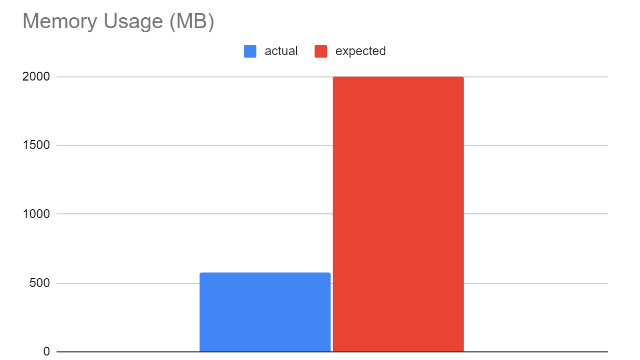
\includegraphics[width=0.5\linewidth]{memuse.png}
    \caption{MEM Use exp v act}
    \label{memuse}
\end{figure}

\begin{figure}
    \centering
    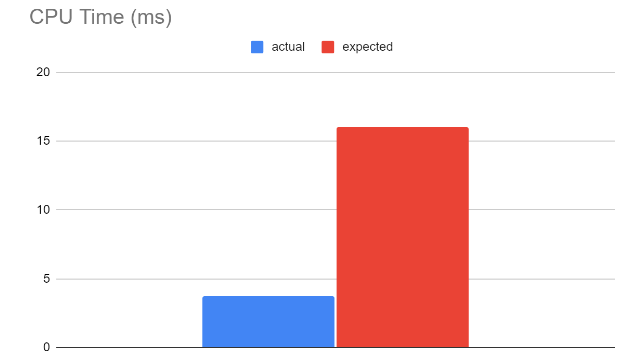
\includegraphics[width=0.5\linewidth]{cputime.png}
    \caption{CPU Time exp v act}
    \label{cputime}
\end{figure}

\begin{figure}
    \centering
    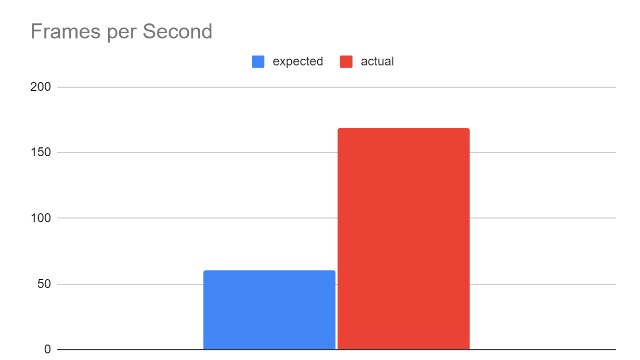
\includegraphics[width=0.5\linewidth]{fps.png}
    \caption{FPS exp v act}
    \label{fps}
\end{figure}

%---------------------------End Product Performance-------------------------------------------------

% No text here.


%---------------------------End Non-Functional Product Details Section---------------------------



% No text here.



%---------------------------Software Product Testing Section-------------------------------------
\section{Software Testing}



%---------------------------Software Testing Plan Template-------------------------------------

\subsection{Software Testing Plan Template}
%Each of the testing levels (unit, Integration, System, Acceptance) should use the following test plan template.

\textbf{Test Plan Identifier:} %Provides a unique identifier for the test. Every test should have a unique identification number for reference.

\textbf{Introduction:} % 50 words minimum. Brief description and objective about the test type.

\textbf{Test item:} %50 words minimum. Includes detailed information about the Software Under Test (SUT).

\textbf{Features to test/not to test:} %50 words minimum. In scope features. This could be newly added or updated features. Out of scope features not tested. [Provide reasoning for exclusion, like, non-impacted, low priority, etc.]

\textbf{Approach:} %50 words minimum. Strategy to test the software. Includes types of tests and how to test. Functional, performance, security testing using combined [manual + automation], manual only, automation only approach.

\textbf{Test deliverables:} %50 words minimum. All the deliverables from the testing e.g. approaches, test cases, reports etc.

\textbf{Item pass/fail criteria:} %50 words minimum. Entry and Exit criteria for all items. 

\textbf{Environmental needs:} %50 words minimum. Infrastructure required for SUT and executing test cases.

\textbf{Responsibilities:} %50 words minimum. Roles and responsibilities for various testing / supported activities.

\textbf{Staffing and training needs:} %50 words minimum. Training needs to bridge the gap of available and expected skill.

\textbf{Schedule:} %50 words minimum.  Test schedule should also be noted in the Gantt Chart. Test estimation (Efforts) and high-level schedule. Schedule should be for key deliverables or important milestones. Ideally, all test deliverables included in the test plan should be scheduled.

\textbf{Risks and Mitigation:} %100 words minimum. Risk identification for applicable items, assumptions, and mitigation plan.

\textbf{Approvals:} %Approvals and sign of dates.

%---------------------------Software Testing Plan Template-------------------------------------


% No text here.



%---------------------------Unit Testing-------------------------------------
\subsection{Unit Testing}
%copy of the completed Unit test plan should be placed here.
Text goes here.

\subsubsection{Source Code Coverage Tests}
%150 words minimum
%Insert Flow Graph Image(s).  Define cyclomatic complexity, basis paths, and Unit Test Cases
Text goes here.

%uncomment the section below when you're ready to insert an image
%\begin{figure}[h!]
%    \centering
%    \includegraphics[width=0.5\textwidth]{images/flow_graph.png}
%    \caption{Description of the image here.}
%    \label{flow_graph}
%\end{figure}



\subsubsection{Unit Tests and Results}
%All unit tests results visualized (table, graph, etc.)
Text goes here.


%---------------------------End Unit Testing-------------------------------------

% No text here.

%---------------------------Integration Testing-------------------------------------
\subsection{Integration Testing}
%copy of the completed Integration test plan should be placed here.
Text goes here.

\subsubsection{Integration Tests and Results}
%All integration tests results visualized (table, graph, etc.)
Text goes here.


%---------------------------End Integration Testing-------------------------------------

% No text here.


%---------------------------System Testing-------------------------------------
\subsection{System Testing}
%copy of the completed System test plan should be placed here.
Text goes here.

\subsubsection{System Tests and Results}
%All system tests results visualized (table, graph, etc.)
Text goes here.


%---------------------------End System Testing-------------------------------------

% No text here.


%---------------------------Acceptance Testing-------------------------------------
\subsection{Acceptance Testing}
%copy of the completed Acceptance test plan should be placed here.
Text goes here.

\subsubsection{Acceptance Tests and Results}
%All Acceptance tests results visualized (table, graph, etc.)
Text goes here.


%---------------------------End System Testing-------------------------------------

% No text here.





%---------------------------End Software Product Testing Section-------------------------------------


% No text here.



%---------------------------Conclusion Section-------------------------------------
\section{Conclusion}
%300 words minimum
%Concluding remarks that summarizes the purpose and outcomes of the technical document.  Discussion of short comings and future work.
Text goes here.

%---------------------------End Conclusion Section-------------------------------------


% No text here.



%---------------------------Appendix Section-------------------------------------------
\section{Appendix}

\subsection{Software Product Build Instructions}
%Include in this section all steps for copying the current state of the product to new computers for continued development.
For continuation of the project, there is a repository made that includes all documentation, assets, and source code. Once the repository has been cloned you can open up the Unity Hub and add a project from disk and go to the github folder and click on the cloned project. Unity Hub should install the correct version of Unity for you and open the project. 

\subsection{Software Product User Guide}
%Include in this section an overview guide on how to use your software product for a general user and an administrative user.
The user experience has been streamlined as the user will have the build product of the game/software already ready for them. Once they open the build with the correct version of Unity, they will be prompted to create a user account, login, and then be able to enjoy the remake of Star Wars SMS edition. Additionally, the build should work on any platform that can run Unity and no additional settings have to be changed in order to do so.

\subsection{Source Code with Comments}
%Include in this section all final source code for the product.  Label each file with headings such as, C.1 file1.c, C.2 file2.c, C.3 file1.py, etc.  All source code should be effectively commented.
https://github.com/mattirizarry/CS360-Project/tree/main/StarWars







%---------------------------End Appendix Section-------------------------------------------














%example image:  uncomment to show usage
%\begin{figure}[h]
%    \centering
%    \includegraphics[width=0.5\textwidth]{images/Add_non-music.png}
%    \caption{This is how you add non-music items.}
%    \label{fig16}
%\end{figure}


%example links:  uncomment to show usage.
%\url{https://www.youtube.com}
%\href{https://www.wku.edu/}{WKU Homepage}
%\footnote{You can put the link in a footnote like this.}

% Anything to the right of a percent sign will be ignored by LaTeX.
% You can use this to put notes to yourself.  



\end{document}
